\documentclass[10pt,a4paper]{article}

\usepackage[top=1in, bottom=1.25in, left=1in, right=1in]{geometry}

%\usepackage[spanish]{babel}
\usepackage[utf8x]{inputenc}

\usepackage{hyperref}

%math packages
\usepackage{amsmath}
\usepackage{amsfonts}
\usepackage{mathtext}

%modify captions
\usepackage[font={footnotesize}, margin = 1.5cm]{caption}

\usepackage{graphicx}
\usepackage{subfig}


\usepackage{parskip}
\setlength{\parskip}{0.5cm} 
\setlength{\parindent}{1cm}

\title{Stochastic Analysis of EEG measures}
\author{
        \small{Xavier Civit \& Pablo Ruiz} \\
         \small{Stochastic Applied Processes}\\
                \small{Universitat Autònoma de Barcelona}
}
\date{\today}

\begin{document}
\maketitle

\begin{abstract}
A brief review of a dual-process model using the replicator equation is presented. This model consists of agents taking decisions based on 
automatic or controlled processing, and compete with each other for survival. This framework will let us describe the long-term state, and 
the conditions under which coexistence, bistability or automatic/control dominance takes place.

With the addition of feedback effects
between the population state and the environment, we were able to observe the appearance of limit cycles, leading the population dynamics
to a persistent oscillatory behaviour. In general, limit cycles only occur when the environment-population feedback time scale is long. It was shown that
the increase of controlled agents in the total population alters the environment in a manner so that automatic agents can start invading the population, and
vice versa. As a personal contribution, a simple nonlinear analysis was made and computer simulations were carried out to represent the dynamics and 
the phase portraits for the different scenarios.
\end{abstract}

\tableofcontents

\section{Introduction}

Experimental setting system is described in \cite{Experiment:BCI2000} and data collection

\section{Artifacts}

Artifacts are mainly due to eye blinking and eye ball movement \cite{EEG:artifacts}

\begin{figure}[h!]
\centering
\vspace{-2cm}
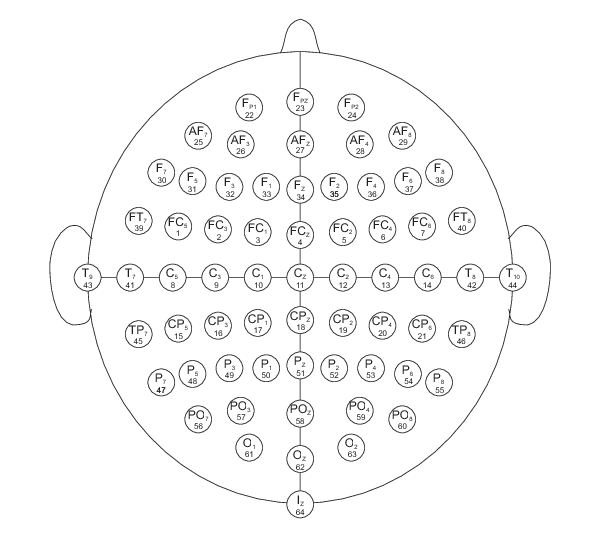
\includegraphics[width=0.6\textwidth]{Figures/64_channel_sharbrough.pdf}
\vspace{-2cm}
\caption{EEG channel setting made by \cite{Experiment:BCI2000}.}
\label{fig:fitness}
\end{figure}




Classical game theory embraces the concept of rational decision making. It gives a theoretical framework to descrive 
agents that are engaged in a given game or interaction with other agents, and have to decide between different strategies.
The decision process of every agent is driven in such a way that it maximizes their payoff, and this payoff depends on the strategies
of the rest of co-agents. Since these frequencies change according to the payoffs, this yields a
feedback loop. Evolutionary game theory studies entire sets of agents that are programmed to use a certain type of
behaviour or strategy \cite{Hofbauer:evolutionary}. 

The use of the evolutionary game theory to describe two-player games has been widely used before since Maynard Smith introduced \cite{Smith:1974} in 1974 
the concept of evolutionary stable strategy. The problem is that stable strategy is a static concept, and it cannot provide an answer on how this 
state is achieved \cite{Silva:2011}. This limitation was overcome by Taylor and Jonker \cite{Jonker:1978} in 1978 by introducing replicator dynamics, and
were able to make a connection between the evolutionary stable strategy concept and the evolutionary equilibrium. In symmetric two player games, every
population state that is an evolutionary stable state is in evolutionary equilibrium in the replicator dynamics. Furthermore, Bomze and Weibull showed 
\cite{Bomze:1995} in 1995 that in symmetric two-player games, every population state that is a neutrally stable strategy is neutrally stable in the replicator
dynamics.

\section{Evolutionary game dynamics}

As presented in  \cite{Hofbauer:evolutionary} and \cite{Hofbauer:deterministic}, we consider a large population of players, with a finite set 
of pure strategies $\{1,...,n\}$. $x_i$ denotes the frequency of strategy $i$. 
$\Delta_n= \{x_i \in\mathbb{R} : x_i \geq 0, \sum_{i=0}^n x_i = 1 \}$ is the $n-1$ dimensional symplex.

The payoff to strategy $i$ in a population $x$ is $a_i (x) $, with $a_i : \Delta_n \rightarrow \mathbb{R}$ being a continuous function that defines our
population game. The most special case is that of a symmetric two person game with $n\times n$ payoff matrix $A = (a_{ij})$; with random mathing this leads to 
the linear payoff function $a_i(x) = \sum_j a_{ij} x_j = (Ax)_i$.

A specific set of strategies $\hat{x}$ are said to be in Nash equilibrium (\cite{Nash:1950} and \cite{Nash:1951}) if 

\begin{equation}
 \hat{x}\cdot a(\hat{x}) \geq x \cdot a(\hat{x}), \; \; \; \forall x \in \Delta.
 \label{eq:nash}
\end{equation}

Moreover, a mixed strategy $\hat{x}\in\Delta$ is an evolutionary stable strategy if (\cite{Jonker:1978}, \cite{Smith:1982}):

\begin{itemize}
 \item $x\cdot A \hat{x} \leq \hat{x}\cdot A \hat{x}$ \hspace{0.6cm} $\forall x \in \Delta, \; \; \; $ and
 \item $x\cdot A x < \hat{x}\cdot A x$ \hspace{0.6cm} for $x\neq\hat{x},$ if there is equality in the previuous point.
\end{itemize}

The first statement is a refined version of the Nash equilibrium. The second statement implies that games satisfying it have a unique
evolutionary stationary state, which also implies that it is the unique Nash equilibrium.

\section{Replicator dynamics}

The differential equation we will now present had already been used in other contexts such as population genetics and chemical networks (see \cite{Hofbauer:1988} or \cite{Hofbauer:1998}
for historical remarks). Following \cite{Ohtsuki:replicator} presentation of the replicator equation, consider an evolutionary game with $n$ strategies, 
labelled $i=1,...,n$. The payoff matrix, $A$, is an $n\times n$ matrix, whose elements $a_{ij}$, denote the payoff for
strategy $i$ versus strategy $j$. The relative abundance (frequency) of each strategy is given by $x_i$. We have $\sum_{i=1}^{n} x_i = 1$. The fitness of strategy $i$ is given 
by $f_i = \sum_{j=1}^{n} x_j a_{ij}$. For the average fitness of the population, we obtain $\phi = \sum_{i=1}^n x_i f_i$. The replicator equation is then given by 

\begin{equation}
\dot{x}_i=x_i(f_i - \phi), \; \; \;  i=1,...,n.
\label{eq:replicator}
\end{equation}

This equation is one of the fundamental equations of evolutionary dynamics. It describes evolutionary game dynamics (frequency dependent selection) in the deterministic
limit of an infinitely large, well-mixed population \cite{Ohtsuki:replicator}. The term "well-mixed" reffers to the fact that all individuals are equally likely to interact with each other,
\emph{i.e.}, the population structure is ignored. As defined in the previous section, this evolutionary equation is defined on the simplex $S_n$. This simplex $S_n$ is invariant
under replicator dynamics, \emph{i.e.}, a simplex trajectory can never leave the simplex. In addition, replicator equation describes pure selection dynamics, so mutation is not considered.
If a strategy is evolutionary stable (strict Nash equilibria, equality in (\ref{eq:nash})), then the corner point of the simplex corresponding to an homogeneous population using this
strategy is an asymptotucallt stable fixed point (\cite{Ohtsuki:replicator}). It can also be proven (\cite{Nowak:book},\cite{Cressman:replicator}) that there can be at most one isolated
equilibrium in the interior of the simplex.

\section{Controlled vs. Automatic Decision-Making}

Dual-system theories of cognition \cite{Cohen:1990, Miller:2001, Posner:1975, Schneider:1977, Shiffrin:1977, Barrett:2006} have focused on explaining
why humans, with our capacity for deliberation and rational thinking, sometimes behave impulsively and succumb to immediate benefits, thus acting against our own 
long-term interest. This theories prupose two types of processes: automatic ones that give fast and effortless typical responses, and controlled ones that take more time
for thinking. 

Studying the interactions between this two kinds of processing could let us understand important problems in different scopes like social problems, ecology
or economics. Important problems we are facing nowadays in our modern world such as shortfalls in retirement savings, increase of obesity and drug addicion, depletion of the environment,
and other seemingly irrational behavior (\cite{Ariely:2008,Loewenstein:1996}). 

Following, we present a model developed by \cite{Strogatz:evolutionary} that describes, in the framework of evolutionary game dynamics, how automatic and controlled agents
compete in a resource world. With a simple analysis we will be able to state different regimes of behaviour for the long-term state of the system.

\section{The Model}

We model our game as a world in which players compete for resources, and they choose how to consume these goods they acquire to generate fitness, with 
fitness being subject to diminishing marginal returns on consumption. Agents are then subject to natural selection based on their resulting fitness \cite{Strogatz:evolutionary}.

For the sake of simplicity, we will assume there are only two types of agents, fully controlled and fully automatic. We will then study the evolution of the 
fraction of controlled agents, denoted by $x$. These agents have the following features that characterize them:

\begin{itemize}
 \item Automatic agents are more efficient and fast to acquire goods
 \item Controlled agents consume resources more "intelligently".
\cite{Simulations:code}
\end{itemize}

Following the same notation as in the original paper \cite{Strogatz:evolutionary}, worlds richness is parametrized by the probability $\rho$ of finding a good,
with all goods being of equal size and normalized to 1 energy unit. The competitive advantage of automatic agents have over controlled agents will be denoted by
$\beta$. For $\beta=0$, agents have same probability of finding a good. This competitive advantage of automatic processing over controlled, will be reflected by
the average waiting time of both types of agents, \emph{i.e.}, the average number of time steps between acquiring one good and the next. If we define a probability
of acquiring a good, $p_A$ for automatic agents and $p_C$ for controlled

\begin{equation}
p_A = \rho(1+\beta x), \; \; \; \; p_C = \rho(1-\beta(1- x))
\label{eq:probability}
\end{equation}

\noindent we can express the average waiting time as the inverse of that probability

\begin{equation}
 \tau_A = \frac{1}{p_A}, \; \; \; \; \tau_C = \frac{1}{p_C}
 \label{eq:tau}
\end{equation}

It is now clear that automatic agents will have a shorter waiting time between consumption, as both $\rho$ and $\beta$ will be greater than zero, $\tau_A < \tau_C$.
An important feature of the model is that for an increasing $x$, both $p_A$ and $p_C$ grow, but the population average probability of finding a resource remains
constant, $x p_C + (1-x)p_A = \rho$. Putting it into words, this happens because as the fraction of controlled $x$ increases, a bigger portion of
population is made up of agents that have a lower probability of acquiring goods, and this reduction in average probability exactly 
balances out the increase in likelyhood of any agent acquiring a resource.

Consumption of resources will be characterized by the fitness of both type of agents. We can define the fitness gained from consuming a fraction $z$ of a good as
$z/(a+z)$, where $a$ determines the quantity of diminishing marginal returns; as $a$ decreases, resources will be consumed faster. As stated previously, goods are
normalized to have size 1.

For automatic agents, once they acquire a good, they consume all of it immediately, thus $z=1$, giving a fitnees benefit of $1/(a+1)$. After this first time step of 
consumption, they spend, on average $\tau_A -1$ time steps consuming nothing, until they acquire a good. Now, we can define their fitness per time step as

\begin{equation}
f_A = \frac{\displaystyle\frac{1}{1+a}}{\tau_A} = \frac{\rho + \beta \rho x}{a+1}
 \label{fittness:a}
\end{equation}

Unlike automatic processing, controlled agents consume gained resources more carufully; their consumption is spaced in time, spreading it out evenly in order to obtain 
the maximum amount of fitness gain from it. It is obvious to note that because of the diminishing marginal returns on cunsumption $a$, it is more beneficial to
pace the cunsumption. This yelds the planned consume of controlled agents to  $z=1/\tau_C$ for every time step $\tau_C$ and thereby the fitness gain per time step, 
using Eqs. (\ref{eq:probability}) and (\ref{eq:tau}) is

\begin{equation}
f_A = \frac{\displaystyle\frac{1}{\tau_C}}{a+\displaystyle\frac{1}{\tau_C}} = \frac{\rho(\beta(x-1) +1)}{a+\rho(\beta(x-1)+1)}
 \label{fittness:c}~
\end{equation}

As it could be expected, $f_A$ is linear with $p_A$, \emph{i.e}, with $x$, and $f_C$, is concave with respecto to $p_C$ (also respect to $x$, of course). Both
functions increase monotonically, and have the shape given by Fig.\ref{fig:fitness}.

\begin{figure}[h!]
\centering
\vspace{-2cm}
\includegraphics[width=0.6\textwidth]{Figures/fitness.pdf}
\vspace{-0.3cm}
\caption{Fitness curves for automatic and controlled processing, $f_A(p_A)$ and $f_C(p_C)$.}
\label{fig:fitness}
\end{figure}

\subsection{Replicator dynamics in a constant environment}

Having translated both automatic and controlled strategies into fitness gains, we are now able to study the whole system as an evolutionary game. We want to know
which strategy, or a combination of the two, will be favoured by natural selection for different values of resoure availability $\rho$ and competitive advantage 
over resources of automatic agents $\beta$. Here is when replicator equation \ref{eq:replicator} comes into play, characterizing how the fractions $x$ and $1-x$ 
vary over time. As the quantity for automatic agents is given by $1-x$, we will only need to present an evolutionary equation for the 
fraction of automatic agents $x$. 
It is convenient to use this approach because the replicator equation will compare the fitness of controlled agents to the population average fitness. Controlled
agents frequency will only grow if their fitness, for a given set of parameters $\{\rho,\beta,a\}$, is higher than the one corresponfing to automatic agents.

Using Eqs. (\ref{eq:replicator}), (\ref{eq:probability}) and (\ref{eq:tau}), the replicator equation for our system is given by

\begin{equation}
\dot{x} = x(f_C - (xf_C+(1-x)f_A)) = x(1-x)\displaystyle\left( \frac{a}{a-\beta\rho+\rho+\beta\rho x} + \frac{\rho+\beta\rho x}{a+1} -1 \right)
 \label{Replicator:master}
\end{equation}

We are now interested in descriving the long-term dynamics of (\ref{Replicator:master}), in terms of the parameters $a$, $\rho$ and $\beta$. It is straight-forward
to see that the end points of our domain are always fixed points, \emph{i.e.}, $x^* = 0$ and $x^* = 1$, regardless of the values of $a$, $\rho$ and $\beta$. 
It can also be infered that the maximum number of fixed points for our system will be 4, since we are dealing with a 4th degree polynomial of $x$. Our bifurcation 
analysis proves that there are 5 distinct regions, depending on the values of our parameters. Computer simulations have also been performed to show the time evolution of the system
for the different scenarios (simulation code adapted from \cite{Simulations:code}).

We will now give a detailed description of different regions. As in the original 
paper \cite{Strogatz:evolutionary}, we will fix $a=0.15$ in order to make it easier to illustrate our portrait:

\begin{itemize}
 \item {\underline{Region 1:} Obviously, the fixed points for this region are $x^*=0$, $x^*=1$. Additionally, we have a third positive root for the right most expression in
       (\ref{Replicator:master}), 
       
 $$x^*=\frac{\beta^2 \rho -2\beta\rho+\beta}{2\beta^2 \rho}.$$
 
 This last point is the root, with multiplicity 2, of the right most expression in (\ref{Replicator:master}). Since the second derivative of $x$ at $x^*$ is negative, we can conclude that $x^*$ will be a stable 
 point, and the phase portrait will be $\circ\rightarrow\bullet\leftarrow\circ$. If we run a simulation, let's say, for $\{a,\rho,\beta\}=\{0.15,0.8,0.4\}$ we
 obtain the following evolution for both $x$ and $x-1$. 
 
\begin{figure}[h!]
\centering
\vspace{-1.5cm}
\includegraphics[width=0.49\textwidth]{Figures/region1a.pdf}
\includegraphics[width=0.49\textwidth]{Figures/region1b.pdf}
\vspace{-0.4cm}
\caption{Time series of solutions in region 1 with  $\{a,\rho,\beta\}=\{0.15,0.8,0.4\}$ with different initial conditions.}
\end{figure}
 
 The characteristics of this region could be translated into words as a rich world, with $\rho$ being sufficiently large, and with relatively weak competitive
 advantage for automatic processing, with $\beta$ being relatively small. Both $p_A$ and $p_C$ are close to 1, since resources $\rho$ are common. For this reason,
 when going from $x=0$ to $x=1$ automatics fitness increases and with the right $\rho$ and $\beta$, control outperforms automatic near $x=0$, as it is rare, but 
 as $x$ increases the advantage of control diminishes and automatic is fitter. Thus, none of the endpoints is stable, and we have coexistence.
 }
 \item {\underline{Region 2:} the only fixed points for this region are the endpoints $x^*=0$, $x^*=1$. Both roots for the right most expression in (\ref{Replicator:master})
	are negative, so we will neglect them. The condition for those roots to be negative is:
	
	$$2\rho\beta > \beta^2\rho + \sqrt{\beta^2 (-2\beta(2a\rho+\rho)+\beta^2\rho^2+1)}.$$
 
 If we analyze the stability of both $x^*=0$ and $x^*=1$, we see that at the first point, $\ddot{x}$ is positive, thus being unstable, and for the second point
 $\ddot{x}$ is negative, thus being stable. This gives the phase portrait $\circ\rightarrow\bullet$. Setting the parameters $\{a,\rho,\beta\}=\{0.15,0.4,0.4\}$ 
 the evolution for $x$ and $x-1$ is the following
 
\begin{figure}[h!]
\centering
\vspace{-1.5cm}
\includegraphics[width=0.6\textwidth]{Figures/region2a.pdf}
\vspace{-0.4cm}
\caption{Time series of a solution in region 2 with  $\{a,\rho,\beta\}=\{0.15,0.4,0.4\}$.}
\end{figure}
 
 When the world is low on resources and the competitive advantage of automatic processing is low, $x^*=1$ is the global attractor and controlled agents 
 dominate over automatic ones. Automatic agents always consume $\rho\beta$ more goods in average than controlled agents for each time step 
 (using (\ref{eq:probability})), but controlled agents make more intelligent use of those resources, as stated by parameter $a$. Thus, for a given value of $a$,
 controll will win when $\rho\beta$ is sufficiently small. Further, We will discuss in more detail how this region resembles region 4, since both will be dominated
 by a type of agent.
 }
 
 \item {\underline{Region 3:} the fixed points for this region are $x^*=0$, $x*=1$ and 
 
$$ x^*= \frac{\beta^2\rho - 2\rho\beta + \beta + \sqrt{\beta^2 (-2\beta(2a\rho+\rho)+\beta^2\rho^2+1)}}{2\beta^2\rho}$$
 
 The fourth root is negative, so we will neglect it. The stability portrait is the oposite for region 1, giving an unstable fixed point for $0<x^*<1$ and two 
 stable for the end points, 0 and 1: $\bullet\leftarrow\circ\rightarrow\bullet$. For conveniance, we will set the parameters $\{a,\rho,\beta\}=\{0.15,0.1,0.95\}$, 
 and we will run a simulation, giving the following evolutionary profile:
 
\begin{figure}[h!]
\centering
\vspace{-1.5cm}
\includegraphics[width=0.49\textwidth]{Figures/region3a.pdf}
\includegraphics[width=0.49\textwidth]{Figures/region3b.pdf}
\vspace{-0.4cm}
\caption{Time series of solutions in region 3 with  $\{a,\rho,\beta\}=\{0.15,0.1,0.95\}$ with different initial conditions.}
\end{figure}
 
 This region can be featured as a poor world ($\rho\rightarrow 0$), with a huge competitive advantage of automatic agents over controlled agents. Obviously, $p_A$
 and $p_C$ are close to zero, so $f_C$ increases more rapidly for control when moving from $x=0$ to $x=1$ and the other way around happens for $f_A$ when moving 
 from $x=1$ to $x=0$. Thus, both endpoints will create a bistally region in our dynamics. 
 }
 
 \item {\underline{Region 4:} as in region 2, the only fixed points for this region are $x^*=0$, $x*=1$. This can be explained because both roots for the right 
 most expression in (\ref{Replicator:master}) are complex. The condition that has to be fulfilled for all three parameters is
 
 $$2\beta\rho(2a+1) > \beta^2\rho^2 +1.$$
 
 Evaluationg $\ddot{x}$ at both endpoints, it arises that for $x^*=0$ $\ddot{x}$ is negative, thus it is global attractor, and $\ddot{x}$ at $x^*=1$ is positive,
 thus giving an unstable fixed point. The stability portait is : $\bullet\leftarrow\circ$. If we run a simulation with $\{a,\rho,\beta\}=\{0.15,0.9,0.9\}$, we
 get the evolution drawn in Fig.\ref{fig:region4}.
 
 In contrast to region 2, we now have a rich world, with high competitive advantage of automatic agents. In this region, automatic outperforms control,
 thus $x=0$ becomes a global attractor. As discussed in region 2, for sufficiently large values of $\rho\beta$, automatic processing will dominate over control. In
 contrast, if $\rho\beta$ is sufficiently small, controlled processing will overpass automatic. Thus, parameter $a$ controlls how large is region 2 compared to 
 region 4: the greater $a$ is, the smaller are the diminishing marginal returns on consumption, thus the larger region 4 is and the smaller region 2 is.

 \begin{figure}[h!]
\centering
\vspace{-1.5cm}
\includegraphics[width=0.6\textwidth]{Figures/region4a.pdf}
\vspace{-0.4cm}
\caption{Time series of a solution in region 4 with  $\{a,\rho,\beta\}=\{0.15,0.9,0.9\}$.}
\label{fig:region4}
\end{figure}
 
 
 }
 
 \item {\underline{Region 5:} aside from endpoints, there are two more fixed points for the system, those arising as real, positive roots from the right most 
 expression of equation (\ref{Replicator:master}). These fixed point solutions are given bellow
 
 $$x^*_{+/-} = \frac{\beta^2\rho - 2\rho\beta + \beta \pm \sqrt{\beta^2 (-2\beta(2a\rho+\rho)+\beta^2\rho^2+1)}}{2\beta^2\rho}.$$
 
 The stability analysis gives stable fixed points as $x=0$ and $x^*_+$, and unstable ones for $x=1$ and $x^*_-$. Thus, the phase portrait is: 
 $\bullet\leftarrow\circ\rightarrow\bullet\leftarrow\circ$. A simulation is ran (Fig.\ref{fig:region5}) for the parameters $\{a,\rho,\beta\}=\{0.15,0.55,0.85\}$.
 
\begin{figure}[h!]
\centering
\vspace{-1.5cm}
\subfloat{\includegraphics[width=0.49\textwidth]{Figures/region5a.pdf}}
\subfloat{\includegraphics[width=0.49\textwidth]{Figures/region5b.pdf}}
\vspace{-2.2cm}
\newline
\subfloat{\includegraphics[width=0.49\textwidth]{Figures/region5c.pdf}}
\vspace{-0.4cm}
\caption{Time series of solutions in region 5 with  $\{a,\rho,\beta\}=\{0.15,0.55,0.85\}$ with different initial conditions.}
\label{fig:region5}
\end{figure}
 
 This dynamics result from having a relatively poor environment $\rho$ with high competitive advantage $\beta$ for automatic agents. The interior stable 
 fixed point will be an attractor and there will be coexistence among the two species. 
 }
\end{itemize}

As stated by authors from article \cite{Strogatz:evolutionary}, we must consider how selection pressure varies based on the population makeup if we want to
understand why a rich world with a low competitive advantage for automatic agents leads to coexistence, while a poor world with high competitive advantage for 
automatics leads to bistability. We can generalize that coexistance accours when a given strategy is at an advantage but it is rare. As we have seen, regardless 
of $\beta$ and $\rho$, an increase in $x$ gives higher values for both automatic and controlled fitness $f_A$ and $f_C$. Fitness function $f_C$ is concave 
(see Fig.\ref{fig:fitness}),
though, and an increase in the fraction $x$ can have different effects on the relative fitness of automatic versus controlled processing depending on $(\rho,\beta)$. 

\begin{figure}[h!]
\centering
\vspace{-1.5cm}
\includegraphics[width=0.8\textwidth]{Figures/stability.pdf}
\vspace{-0.4cm}
\caption{Stability diagram of equation (\ref{Replicator:master}) for $a=0.15$. Black curves are transcritical bifurcations, and the purple curve separating regions 4 and 5
is a saddle-node bifurcation. This curves have been plotted using the analysis made in the previous points.}
\label{fig:stability}
\end{figure}
 
As a final remark for this simple model, it is worth noting that as parameter $a$ increases, the space where automatic agents dominate, region 4, will grow and
regions 1,2,3 and 5 will decrease. A stability diagram has been drawn (Fig.\ref{fig:stability}), using the restrictions listed for all previous regions, and
setting the $a$ parameter to 0.15. 

\subsection{Replicator dynamics in a responsive environment}

In the previous section, we modelled the enviornment having a constant behaviour, \emph{i.e}, both $\rho$ and $\beta$ didn't change with time. In the sections
that follow, we will account for the feedback between the population and the enviornment, by introducing a dynamic equation for both $\beta$ and $\rho$. We
will study such systems separately, first introducing an evolutionary equation for the competitive advantage $\beta$. In the following section we will analyze
the effects on the resource availability $\rho$. In the final section we will study the system with a feedback accounting for both features, $\rho$ and $\beta$. 

\subsubsection{Controlled processing increases competitive advantage of automaticity}

We want to model a scenario in which an increase in $x$ will lead to a greater population density, by allowing $\beta$ to grow with $x$. This feature
can be thought as a situation in which rational thinking allows people to live more densely without violent conflict. We will introduce a new 
equation for $\beta$, linking its evolution with $x$ by pulling its value to the current value of $x$. To make it more realistic, a lag is introduced, 
$\tau_{\beta}$, to capture the fact that an increase in $x$ at time $t$ doesn't have an immediate impact on $\beta$. For instance, as stated by 
\cite{Strogatz:evolutionary}, in real life, an increase in 
the birth rate does no lead immediately to a larger number of competing adults. Finally, our system consists of the old equation (\ref{Replicator:master}) plus
the evolution of $\beta$

\begin{equation}
\begin{array}{lcl}
\dot{x} & = & x(1-x)\displaystyle\left( \frac{a}{a-\beta\rho+\rho+\beta\rho x} + \frac{\rho+\beta\rho x}{a+1} -1 \right)\\
\dot{\beta} & = & \displaystyle\frac{x-\beta}{\tau_{\beta}}
\end{array}
\label{eq:master_2}
\end{equation}

We see that in equilibrium, $x=\beta$. The bifurcation analysis made by \cite{Strogatz:evolutionary} gives 3 separete regions for the stationary state of the 
system. We are now going to present them and numerically simulate the evolution of the system. To characterize how this new feature of feedback between the population
and the environment ($\beta$), we fix $a=0.8$ so we can handle with the parameter space $(\rho,\tau_{\beta})$.

\begin{itemize}
 \item {\underline{Region 1:} for sufficiently small values of $\rho$, regardless of $\tau_{\beta}$ there's no interior fixed point and $x^* = 1$ is the global attractor.
 Only if the starting population consists all of it of automatic agents, the stationary solution will be different from $x=1$. The phase portrait for this $(\rho,\tau_{\beta}$ 
 is represented in the first plot of Fig.\ref{fig:portrait_2}. Letting the system evolve, the profile in Fig.\ref{fig:scenario2a} is achieved.  

\begin{figure}[h!]
\centering
\vspace{-2.0cm}
\includegraphics[width=0.6\textwidth]{Figures/scenario2a.pdf}
\vspace{-0.4cm}
\caption{Time series of a solution in region 1, with  $\{a,\rho,\tau_{\beta}\}=\{0.8,0.1,400\}$.}
\label{fig:scenario2a}
\end{figure}
}

 \item {\underline{Region 2:} after a deep analysis made by \cite{Strogatz:evolutionary} it is found that for a certain range of $\rho$ and $\tau_{\beta}$ 
 limit cycles are born in a supercritical Hopf bifurcation. Specifically, limit cycles exist if $0.1<\rho<0.52$ and $\tau_{\beta}>104.47$. The phase portrait of
 these limit cycles is represented in the second plot from Fig.\ref{fig:portrait_2}. If we fix $\rho=0.2$, and run a numerical simulation, we achieve the 
 shape represented in Fig.\ref{fig:scenario2b}.
 
\begin{figure}[h!]
\centering
\vspace{-2.0cm}
\includegraphics[width=0.6\textwidth]{Figures/scenario2b.pdf}
\vspace{-0.4cm}
\caption{Time series of a solution in region 2, with  $\{a,\rho,\tau_{\beta}\}=\{0.8,0.2,400\}$. Limit cycles appear.}
\label{fig:scenario2b}
\end{figure}
}

 \item {\underline{Region 3:} an interior fixed point is found for this region, and both endpoints will result in unstable fixed points. This will lead the 
 dynamics of the system to initially oscilate and then relax to a coexistence point (phase portrait is sketched in the third plot of Fig.\ref{fig:portrait_2}). 
 Parameter $\rho$ must be set greater than 0.52 to avoid the Hopf asymptote (see \cite{Strogatz:evolutionary}). We have also ran a numerical simulation for the dynamics 
 of this region in Fig.\ref{fig:scenario2c}.
 
\begin{figure}[h!]
\centering
\vspace{-2.0cm}
\includegraphics[width=0.6\textwidth]{Figures/scenario2c.pdf}
\vspace{-0.4cm}
\caption{Time series of a solution in region 3, with  $\{a,\rho,\tau_{\beta}\}=\{0.8,0.65,400\}$, leading to coexistence.}
\label{fig:scenario2c}
\end{figure}
}

\end{itemize}

We have seen that for sufficiently large values of $\tau_{\beta}$ and in a specific range of $\rho$, limit cycles appear, meaning that for a sufficiently delayed effect of the
feedback effect, oscillatory dynamics will emerge. Otherwise coexistence will appear and the system will relax. By characterizing the $(a,\rho)$ space, one can find that
the long term dynamics are

\begin{itemize}
 \item If $\rho<(a+1)/2$, dominance of controlled agents (region 1).
 \item If $\rho>(a+1)/2$ and $\rho > \rho^*$, coexistence (region 3).
 \item If $\rho>(a+1)/2$ and $\rho < \rho^*$, limit cycles (region 2.
\end{itemize}

\begin{figure}[h!]
\centering
%\vspace{-1.5cm}
\includegraphics[width=0.3\textwidth]{Figures/reg1.pdf}
\includegraphics[width=0.3\textwidth]{Figures/reg2.pdf}
\includegraphics[width=0.3\textwidth]{Figures/reg3.pdf}
\vspace{-0.4cm}
\caption{Phase portrait $(\beta,x)$ of the three different dynamics of the system. From left to right: control dominance, limit cycles and coexistence.}
\label{fig:portrait_2}
\end{figure}

\subsubsection{Controlled processing increases resource availability}

If we think on the influence that a growing controlled population would have in the environment, it is reasonable to aknowledge that it would enrich it.
In a real world scenario, an increase in resource availability could be created by advances in technology. In this section we will discuss the efect that
controlled agents $x$ have on $\rho$. As in the previous section, we will add a lag term $\tau_{\rho}$ accounting for the non immediate effect, it represents
the time required for that technological change to take place. Thus, our system can be described by the following equations

\begin{equation}
\begin{array}{lcl}
\dot{x} & = & x(1-x)\displaystyle\left( \frac{a}{a-\beta\rho+\rho+\beta\rho x} + \frac{\rho+\beta\rho x}{a+1} -1 \right)\\
\dot{\rho} & = & \displaystyle\frac{x-\rho}{\tau_{\rho}}
\end{array}
\label{eq:master_3}
\end{equation}

The first equation in (\ref{eq:master_3}) is the same one used before, and the only addition is the time evolutionary equation for $\rho$. Again, in equilibrium,
$\rho = x$ holds. In order to ease the analysis, $a$ is set to 1.5, and we examine the different dynamics as a function of $\beta$ and $\tau_{\rho}$. Similarly to the previous 
example, three types of dynamics are observed, but in this case, region dominated by controlled agents is this turn dominated by automatic processing. 

\begin{itemize}
 \item {\underline{Region 1:} for sufficiently small values of $\beta$, regardless of $\tau_{\beta}$ there's an interior fixed that acts as a global attractor. Thus, in this 
 region, both populations will coexist. The phase portrait has been drawn in the first plot of Fig.\ref{fig:portrait_3}. Setting the parameter $\beta=0.2$ and $\tau_{\rho}=1000$, 
 the dynamics plotted in Fig.\ref{fig:scenario3a} is achieved.

\begin{figure}[h!]
\centering
\vspace{-2.0cm}
\includegraphics[width=0.6\textwidth]{Figures/scenario3a.pdf}
\vspace{-0.4cm}
\caption{Time series of a solution in region 1, with  $\{a,\beta,\tau_{\rho}\}=\{1.5,0.2,1000\}$, leading to coexistence.}
\label{fig:scenario3a}
\end{figure}
}

 \item {\underline{Region 2:} similar to the scenario described by eq. (\ref{eq:master_2}), limit cycles are born in  a supercritical Hopf bifurcation, which bounds the limit 
 where coexistance and oscillations occur. Specifically, limit cycles will appear only if $0.249<\beta<0.4$ and $\tau_{\rho}>446.3$. 
 The phase portait for this type of dynamics is represented in the second plot of Fig.\ref{fig:portrait_3}. We now run a simulation fixing $\beta=0.3$, and observe the results
 (Fig.\ref{fig:scenario3b}).
 
\begin{figure}[h!]
\centering
\vspace{-2.0cm}
\includegraphics[width=0.6\textwidth]{Figures/scenario3b.pdf}
\vspace{-0.4cm}
\caption{Time series of a solution in region 2, with  $\{a,\beta,\tau_{\rho}\}=\{0.8,0.3,1000\}$. Limit cycles appear.}
\label{fig:scenario3b}
\end{figure}
}

 \item {\underline{Region 3:} no interior fixed point is found for this region, and automatic agents will overtake control. Obvisouly, the $\beta$ parameter has to be larger
 than the right Hopf asymptote in $\beta^*=0.4$. No matter what's the feedback lag $\tau_{\rho}$ automatic agents will dominate for sufficiently large values of $\beta$. In other
 words, for enough fitten automatic agents, there will be no ballance possible for controlled agents trying to enrich the environment. The time evolution of this dynamics has been
 plotted in Fig.\ref{fig:scenario3c}.
 
\begin{figure}[h!]
\centering
\vspace{-2.0cm}
\includegraphics[width=0.6\textwidth]{Figures/scenario3c.pdf}
\vspace{-0.4cm}
\caption{Time series of a solution in region 3, with  $\{a,\beta,\tau_{\rho}\}=\{0.8,0.45,1000\}$, leading to coexistence.}
\label{fig:scenario3c}
\end{figure}
}

\end{itemize}

Despite the similarities found with the previous scenario, where controlled agents increased competitive advantage of automatics, a major difference has been found. When $x$ and
$\beta$ where positively correlated, only dominance of control was possible, whereas in this later scenario, only automatic agents can dominate. A further analysis made 
in the original paper \cite{Strogatz:evolutionary}, states that the dynamics of (\ref{eq:master_3}), depend deeply on the $a$ parameter. It was found that for $a<1$, 
the evolution of the system is very sensitive to the initial conditions, giving rise to new regions beside the main 3 we have previously described. In summary, we have seen
that adding a feedback between $x$ and the environment also gives rise to limit cycles. In contrast to the previous studied scenario, this happens for a smaller
range of $(\beta,a)$  combinations.

\begin{figure}[h!]
\centering
%\vspace{-1.5cm}
\includegraphics[width=0.3\textwidth]{Figures/reg1_2.pdf}
\includegraphics[width=0.3\textwidth]{Figures/reg2_2.pdf}
\includegraphics[width=0.3\textwidth]{Figures/reg2_3.pdf}
\vspace{-0.4cm}
\caption{Phase portrait $(\rho,x)$ of the three different dynamics of the system. From left to right: coexistence, limit cycles and automatic dominance.}
\label{fig:portrait_3}
\end{figure}

\subsubsection{Controlled processing increases both competition and resource availability}

In the end, we will add both environmental feedback effects to the original equation (\ref{Replicator:master}), having a system of three differential equations

\begin{equation}
\begin{array}{lcl}
\dot{x} & = & x(1-x)\displaystyle\left( \frac{a}{a-\beta\rho+\rho+\beta\rho x} + \frac{\rho+\beta\rho x}{a+1} -1 \right)\\
\dot{\beta} & = & \displaystyle\frac{x-\beta}{\tau_{\beta}}\\
\dot{\rho} & = & \displaystyle\frac{x-\rho}{\tau_{\rho}}
\end{array}
\label{eq:master_4}
\end{equation}

By simulating this dynamics numerically, we have observed that for sufficiently large values of $\tau_{\rho}$ and $\tau_{\beta}$, limit cycles appear (Fig.\ref{fig:scenario4a}).

\begin{figure}[h!]
\centering
\vspace{-2.0cm}
\includegraphics[width=0.6\textwidth]{Figures/scenario4a.pdf}
\vspace{-0.4cm}
\caption{Simulation of (\ref{eq:master_4}), with  $\{a,\tau_{\beta},\tau_{\rho}\}=\{1.5,1000,1500\}$, leading to the appearance of limit cycles.}
\label{fig:scenario4a}
\end{figure}

\section{Conclusions}\label{conclusions}

We have studied a model in which dual-process agents forage for goods in a given environment. Agents using automatic processing have an advantage when acquiring goods, whereas
controlled agents make a more judicious consumption of those goods. By parametrizing the availability of resources as $\rho$ and the competitive advantage of controlled agents 
by $\beta$, we were able to characterize what combinations of the $(\rho,\beta)$ space would lead the system to bistability, coexistance, dominance of control or automatic, and
the those that would let limit cycles arise.

For a constant environment, the general conclusions that can be taken are that natural selection favours controlled agents when both $\beta$ and $\rho$ are small (poor wold with 
low competition), automatic agents when $\beta$ and $\rho$ are large (rich world with high competitive advantage for automatics), bistability when $\rho$ is small and 
$\beta$ large (poor world with high competition) and coexistence when $\rho$ is large and $\beta$ is small (rich world with low competition).

For a changing environment, though, a new feature was observed; for sufficiently large lag values for the feedback effects, limit cycles could be observed. This behaviour 
could not be expected in a simple two-species model, where the game parameters are fixed and only the population fractions vary over time \cite{Nowak:book,Hofbauer:book}.

We can consider, as a naive assumption, taking the limiting case of entirely automatic agents competing against entirely controlled agents. In reality, 
agents exist in a continuum of controlled vs. automatic processing. We have also simplified the consumption mechanism of both agents, giving the automatic agent
an instantaneous consumption and the controlled an evenly paced consumption. This rough simplifications, though, has let us deal with a tractable set of equations that
could be studied analytically to some degree of detail. 
Previous work \cite{Tomlin:article} made by one of the coauthors of the original paper \cite{Strogatz:evolutionary} using computer simulations,
was a back-up for them to develop this analytical model. 

An interesting remark made by the authors of this model is that it demonstrates how tendency for controlled processing to enrich the environment or grow the population
undermines the advantage of controlled cognition, leading to an eventual invasion of automaticity and short-sightedness. This could explain how historical cycles
oscilate through technological advances and planned economy to a more short-term gain planification. In their words, \emph{the success of controlled cognition naturally leads 
to its own demise}.

\bibliographystyle{unsrt}

\bibliography{references}

\end{document}